\documentclass{beamer}

%%%%%%%%%%%%%%% Most of this is sample presentation is from the Research Institute of MIT

%%%%%%%%%%%%%%% Here are some of the themes.  you can experiment with which ones you like.  There may be more than this as well.
%\usetheme{default}
%\usetheme{AnnArbor}
%\usetheme{Antibes}
%\usetheme{Bergen}
%\usetheme{Berkeley}
%\usetheme{Berlin}
%\usetheme{Boadilla}
%\usetheme{CambridgeUS}
%\usetheme{Copenhagen}
\usetheme{Darmstadt}
%\usetheme{Dresden}
%\usetheme{Frankfurt}
%\usetheme{Goettingen}
%\usetheme{Hannover}
%\usetheme{Ilmenau}
%\usetheme{JuanLesPins}
%\usetheme{Luebeck}
%\usetheme{Madrid}
%\usetheme{Malmoe}
%\usetheme{Marburg}
%\usetheme{Montpellier}
%\usetheme{PaloAlto}
%\usetheme{Pittsburgh}
%\usetheme{Rochester}
%\usetheme{Singapore}
%\usetheme{Szeged} %\usetheme{Warsaw}

\usepackage{verbatim}
\usepackage{xcolor}
\usepackage{amsmath}
\usepackage{amsfonts}
\definecolor{light-gray}{gray}{.7}
\newcommand{\mat}[1]{\mathbf{#1}}

\title{Component Analysis V. Sobol Analysis}
\subtitle{(What I've been working on in Matlab)}

\date{}


\begin{document}

%%%%%%%%%%%%%% You make slides with \begin{frame} ... \end{frame}

\begin{frame}
\titlepage
\end{frame}
\addtocounter{framenumber}{-1}

\section{Introduction}
\begin{frame}{System Notation}
\begin{align}
\dot{\vec{x}}&=M\vec{x} \\
\begin{bmatrix}
	\dot{\vec{x}}_1 \\
	\dot{\vec{x}}_2 \\
	\dot{\vec{x}}_3 \\
	\vdots
\end{bmatrix} &= 
\begin{bmatrix}
	A_1 & B_{1,2} & B_{1,3} & \ldots\\
	B_{2,1} & A_2 & B_{2,3} & \ldots\\
	B_{3,1} & B_{3,2} & A_3 & \ldots\\
	\vdots & \vdots & \vdots &\ddots
\end{bmatrix}
\begin{bmatrix}
	\vec{x}_1 \\
	\vec{x}_2 \\
	\vec{x}_3 \\
	\vdots
\end{bmatrix}
\end{align}
If $B$ matrices are all 0 we have a series of completely independent linear systems.

If $B$ matrices are sparse, we have ``compartments'' that are connected to form the overall system.
\end{frame}

\begin{frame}{Parameter Notation}
zoom in on one of those compartments and define parameters	
\begin{align}
	\dot{\vec{x}}_i&=A_i(\vec{\theta})\vec{x_i}\\
	\begin{bmatrix}
		\dot{y}_1 \\
		\dot{y}_2 \\
		\dot{y}_3 \\
		\vdots
	\end{bmatrix} &= 
	\begin{bmatrix}
		\theta_1 a_{1,1} & a_{1,2} & \theta_2 a_{1,3} & \ldots\\
		a_{2,1} & a_{2,2} & a_{2,3} & \ldots\\
		\theta_3 a_{3,1} & a_{3,2} & \theta_2 a_{3,3} & \ldots\\
		\vdots & \vdots & \vdots &\ddots
	\end{bmatrix}
	\begin{bmatrix}
		y_1 \\
		y_2 \\
		y_3 \\
		\vdots
	\end{bmatrix}
\end{align}
locations of $\theta_i$ would depend upon actual model
\end{frame}

\begin{frame}{Two Approaches for Model Reduction}
	Sobol
	\begin{itemize}
		\item Assume $\theta_i\sim U[0.9,1.1]$
		\item Pick number of samples to evaluate, $N_{Sobol}$
		\item Compute Sobol index ($S_i$) and total Sobol index ($ST_i$) of each parameter 
	\end{itemize}
	
	Component
	\begin{itemize}
		\item Run model normally: $\dot{\vec{x}}=M(\vec{\theta})\vec{x}$
		\item Run model without one component: $\dot{\vec{x}}=M(\vec{\theta})\vec{x}, \theta_i=0$
		\item Quantify how much these two runs differ ($C_i$)
		\item Repeat for all components $i=1,2,\ldots,N_\theta$
	\end{itemize}
	
	~\\
	
Want to show that small $S_i$ or $ST_i$ $\nRightarrow$ $C_i$ small
\end{frame}

\section{Matlab Code}
\begin{frame}{Building the system}
	inputs: $[N_1,N_2,\ldots]$, $I_{max}$, $I_{min}$, $N_{connections},x_{total}$
	
	~\\
	
	outputs: $\begin{bmatrix}
		A_1 & B_{1,2} & B_{1,3} & \ldots\\
		B_{2,1} & A_2 & B_{2,3} & \ldots\\
		B_{3,1} & B_{3,2} & A_3 & \ldots\\
		\vdots & \vdots & \vdots &\ddots
	\end{bmatrix},\vec{x_0}$	
	
	with
	
	$A_i\in\mathbb{R}^{N_i \times N_i}$ \\
	$a_{i,j}, b_{i,j} \in \mathbb{Z} \cup [I_{min},I_{max}] \quad \quad a_{i,j} = - a_{j,i}  \quad \quad B_{i,j}=-B_{j,i}^T$\\
	$\sum_{i,j} ||B_{i,j}||_0 = N_{connections}$ \\
	$||\vec{x_0}||_1=x_{total} \quad \quad |\vec{x_0}|=\vec{x_0}$
\end{frame}

\begin{frame}{Building the system}
	Example matrices: 
	
	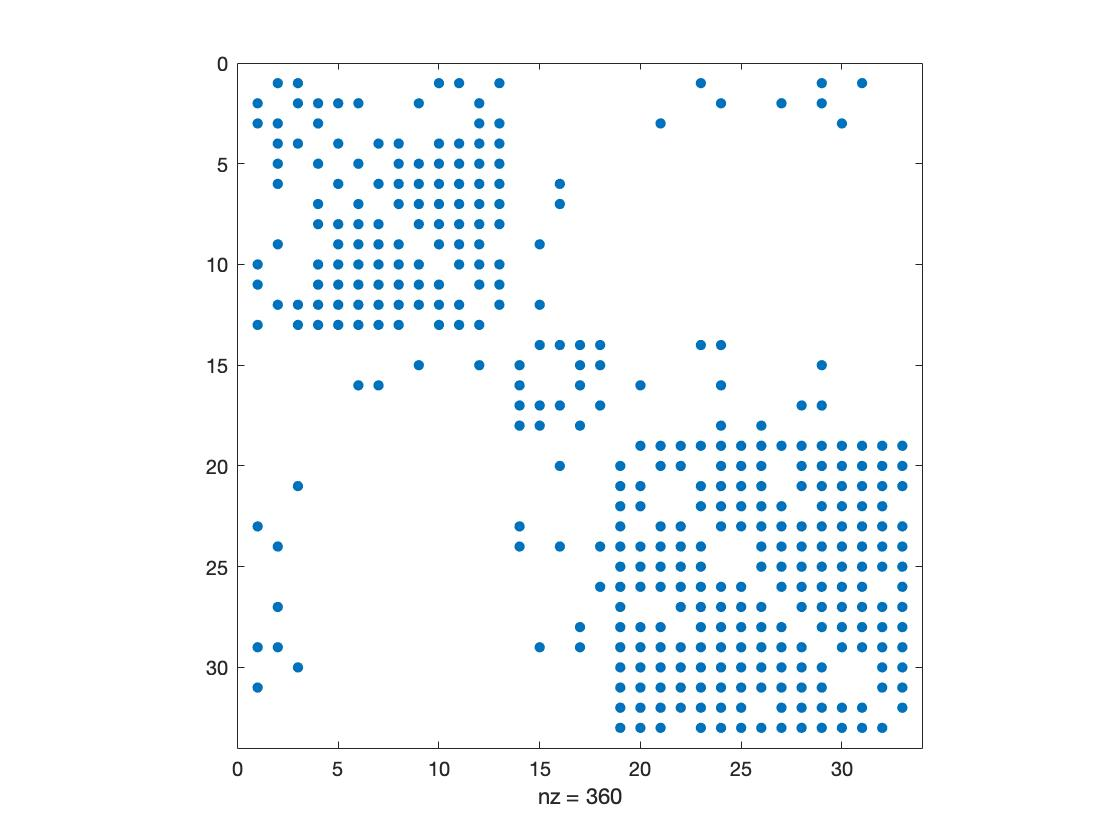
\includegraphics[width=0.49\textwidth]{spy_1.jpg}
	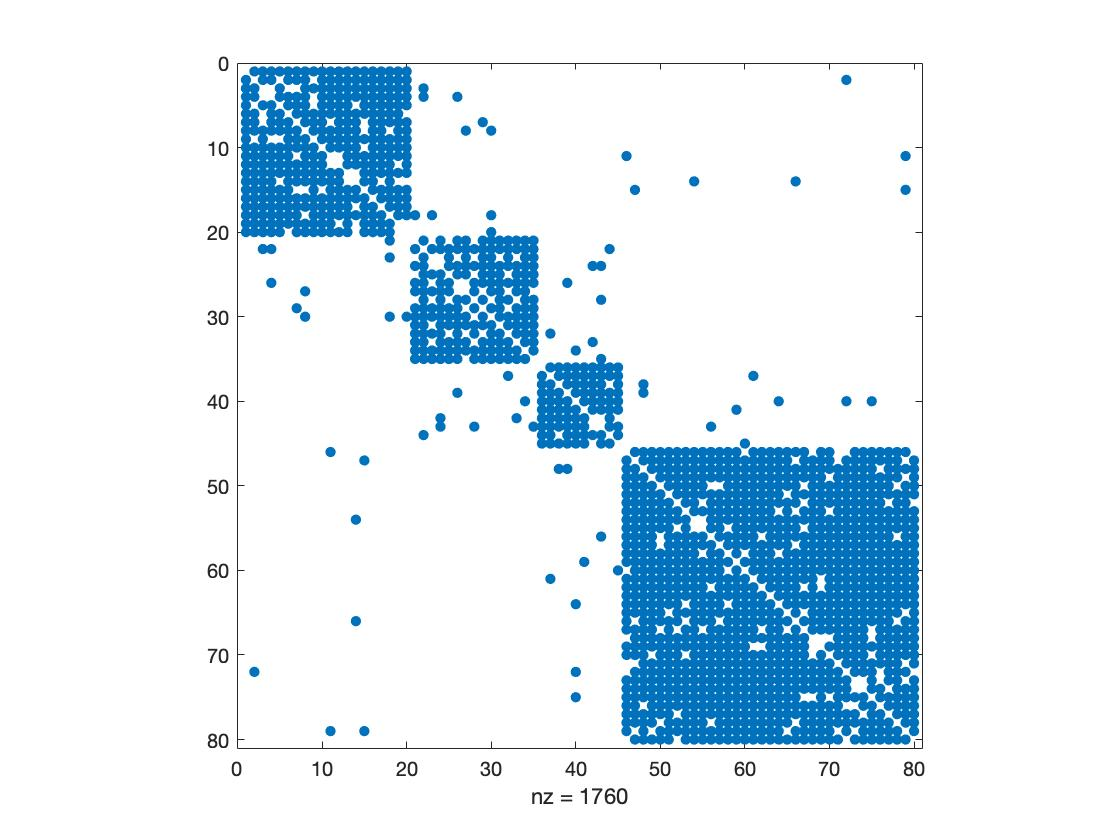
\includegraphics[width=0.49\textwidth]{spy_2.jpg}
\end{frame}

\begin{frame}{Selecting Parameters}
	inputs: $N_{\theta in}$,$N_{\theta out}$ \quad \quad \quad \quad $N_\theta=N_{\theta in}+N_{\theta out}$
	
	~\\
	
	outputs: list of indexes $[i,j]$ to be treated as parameters
	
	with
	
	$N_{\theta in}$ parameters chosen ``inside" compartments \\
	$N_{\theta out}$ parameters chosen ``outside" compartments \\
	All parameters non-zero elements of $M$
	
	~\\
	
	$^\star$currently parameters continue skew symmetry of $M$
	
\end{frame}


\begin{frame}{Selecting Parameters}
	\centering
	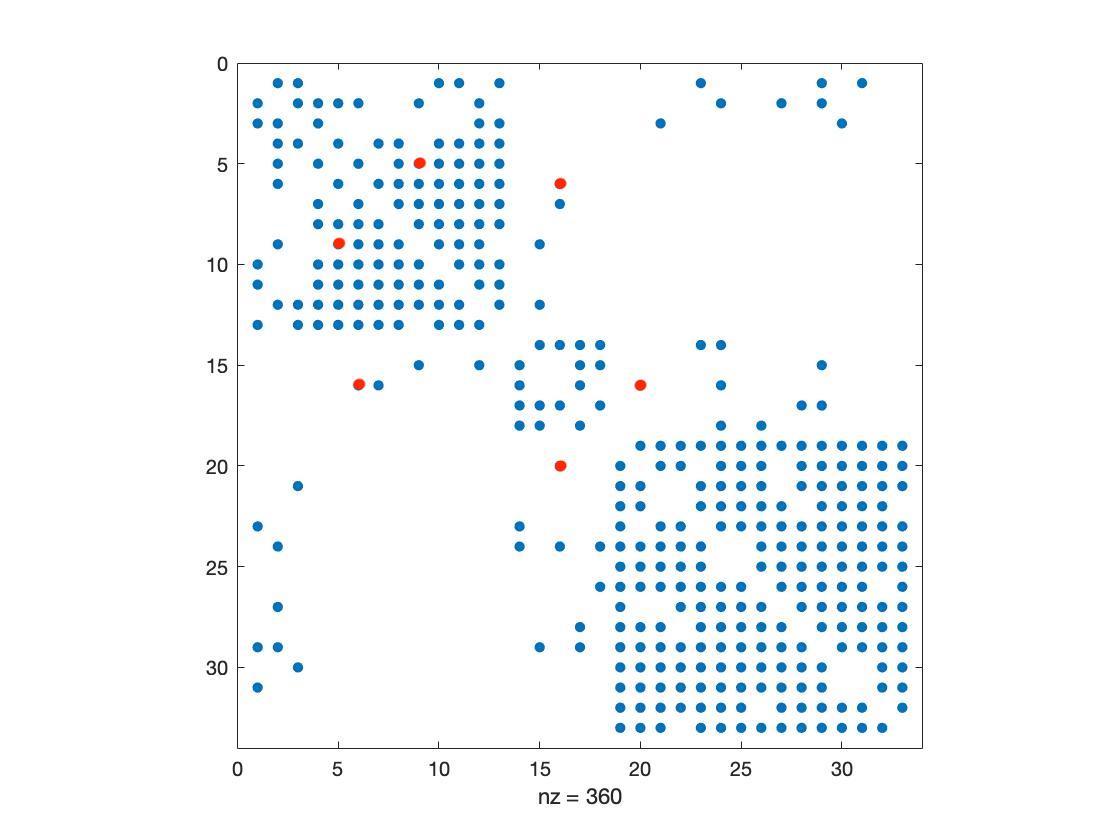
\includegraphics[width=0.8\textwidth]{spy_1b.jpg}
\end{frame}

\begin{frame}{Running the Analysis 1}
	QoI = final value of final state variable
	
	~\\
	
	Component Analysis: $C_i=\frac{|\text{nominal QoI} - \text{altered QoI}|}{\text{nominal QoI}}$
	
	~\\
	
	rank parameters by increasing $C_i$ and increasing $ST_i$, compare lists
\end{frame}

\begin{frame}{Running the Analysis 1}
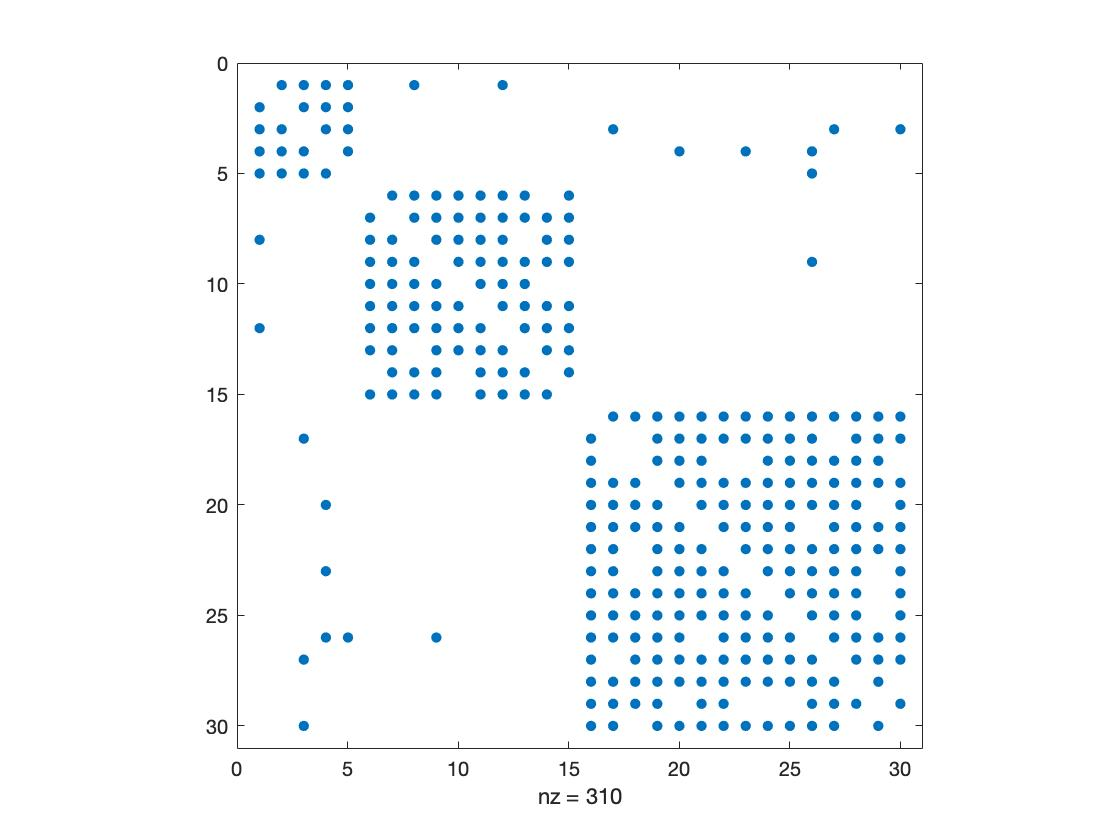
\includegraphics[width=\textwidth]{spy3.jpg}
\end{frame}

\begin{frame}{Running the Analysis 1}
	\centering
\begin{tabular}{|c|c|c|c|}
	\hline
	Parameter & Ranking by C & Ranking by S & Ranking by ST \\
	\hline
	inside 1 & 7 & 10 & 10 \\
	\hline
	inside 2 & 5 & 5 & 4 \\
	\hline
	inside 3 & 8 & 7 & 9 \\
	\hline
	inside 4 & 2 & 3 & 3 \\
	\hline
	inside 5 & 9 & 6 & 5 \\
	\hline
	outside 1 & 1 & 8 & 6 \\
	\hline
	outside 2 & 6 & 9 & 8 \\
	\hline
	outside 3 & 4 & 2 & 2 \\
	\hline
	outside 4 & 10 & 4 & 7 \\
	\hline
	outside 5 & 3 & 1 & 1 \\
	\hline
\end{tabular}
\end{frame}


\begin{frame}{Running the Analysis 2}
	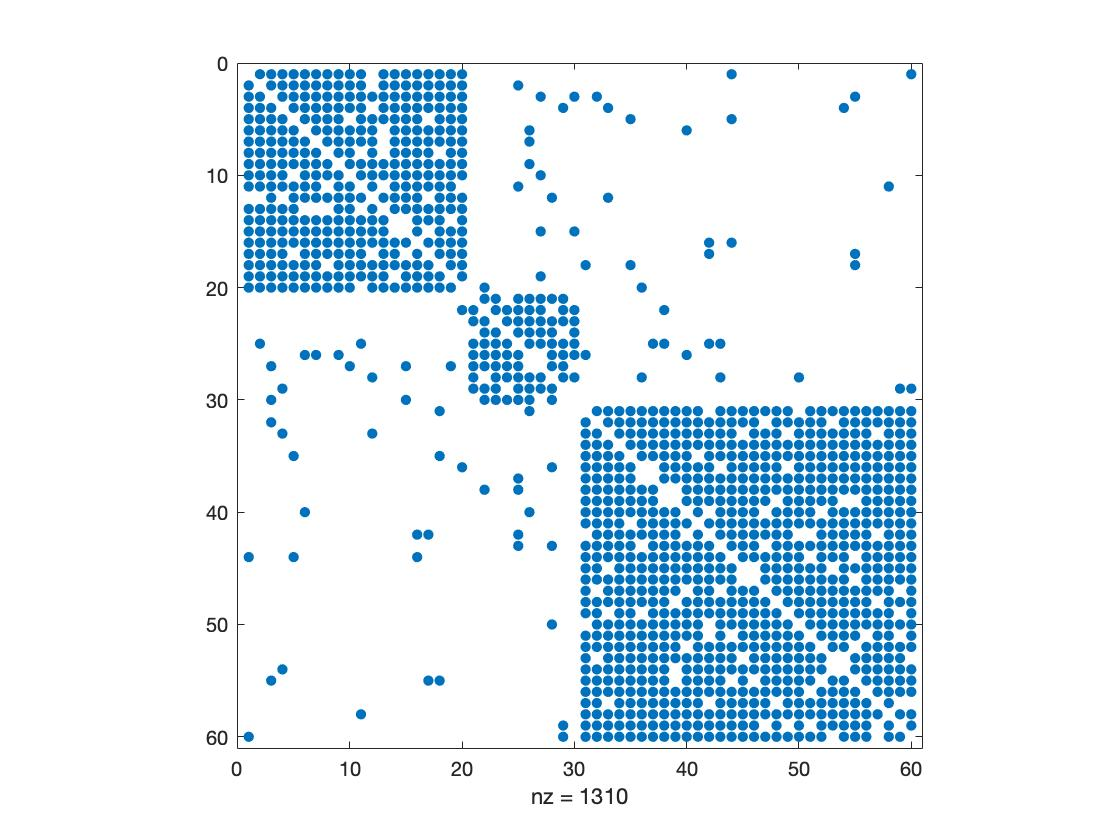
\includegraphics[width=\textwidth]{spy4.jpg}
\end{frame}


\begin{frame}{Running the Analysis 1}
	\centering
	\begin{tabular}{|c|c|c|c|}
		\hline
		Parameter & Ranking by C & Ranking by S & Ranking by ST \\
		\hline
		inside 1 & 3 & 7 & 7 \\
		\hline
		inside 2 & 1 & 2 & 3 \\
		\hline
		inside 3 & 8 & 8 & 8 \\
		\hline
		outside 1 & 7 & 10 & 9 \\
		\hline
		outside 2 & 10 & 6 & 6 \\
		\hline
		outside 3 & 4 & 3 & 2 \\
		\hline
		outside 4 & 2 & 9 & 10 \\
		\hline
		outside 5 & 6 & 1 & 1 \\
		\hline
		outside 6 & 9 & 5 & 5 \\
		\hline
		outside 7 & 5 & 4 & 4 \\
		\hline
	\end{tabular}
\end{frame}

\begin{frame}{Questions}
	\begin{itemize}
		\item Keep parameters mirrored?
		\item Keep M skew-symmetric? ($\dot{\vec{x}}=Me^{-t}\vec{x}$)
		\item $C_i$ computed using all state variables (inner-outer norm)
		\item How to compare different systems? (Distributions)
		\item DIfferent QoI?
	\end{itemize}
\end{frame}

\end{document}